\documentclass[12pt,reqno]{amsart}
\usepackage[margin = 1.0in, footskip=0.35in]{geometry}
%\usepackage{times}
\geometry{letterpaper}
\renewcommand{\baselinestretch}{1.2}
\usepackage{amsmath}
\usepackage{amsthm}
\usepackage{amsfonts}
\usepackage{amssymb}
\usepackage{graphicx}
\usepackage{amssymb}
\usepackage[all]{xy}
\usepackage{epstopdf}
\usepackage{float}
\usepackage{graphicx}
\usepackage{subcaption}
\usepackage{listings}
\usepackage[final]{pdfpages}
\usepackage{ragged2e}
\usepackage[none]{hyphenat}
\usepackage{parskip}
\usepackage{fancyhdr}
\usepackage[english]{babel}
\usepackage[backend = bibtex, maxbibnames = 99]{biblatex}
\addbibresource{spbib.bib}
\pagestyle{plain}
\graphicspath{{Graphs/}, {Figures/}}

\begin{document}
	\begin{center}
    	{MATH 381 Project 2 Autumn 2016\par}
    	\vspace{3 cm}
	    {\LARGE \bfseries Monte Carlo Simulation of Photosynthesis\par}
	    \vspace{11 cm}
	    {\bfseries Group 8\par}
	    \vspace{0.5 cm}
	    {\bfseries James Collins, Baihan Lin, Cheng Peng, Yizhou Yao\par}
	    \vspace{0.5cm}
	    {University of Washington\par}
	    \vspace{0.5cm}
	    {\today\par}
	\end{center}
	
	\newpage
	
	\section*{\large \textbf{Introduction}}
	
	Photosynthesis is one of the fundamental processes of complex life. 
	Without photosynthesis, there would be no life on the Earth.  
	Photosynthesis is also the only process to transfer the solar 
	energy to chemical energy we consume every day. We are 
	interested in how the chemistry of this process works based on the
	available levels of light and the atmospheric composition. 
	To investigate this process, we used a version of Monte Carlo 
	simulation to explore the relationship between the inputs to the 
	reaction and its overall production of glucose, which is used
	later in the metabolic pathway to produce more plant matter. Our model
	makes many simplifying assumptions, but still captures many important
	features of the large-scale reaction kinetics.
	
	Our model examines the process of C3 photosynthesis, the version
	of the reaction common "to approximately 95\% of Earth's plant 
	biomass"\cite{C3_wiki}, including many of the important food crops
	like rice and barley. In our model, we first looked
	for steady state solutions where the process runs without depletion
	of its chemical reserves, characteristic of the plant growing in 
	optimal conditions. Then, we study the effects of perturbations
	to this this steady state to understand how this process is 
	affected by different amounts of sunlight and different $CO_2$
	and $O_2$ composition in the air by examining their impact on the rate 
	of glucose production.
	
	%Furthermore, we 
	%wish to conduct a time-dependent perturbation where we 
	%consider how long and short term sunlight level patterns 
	%influence photosynthesis. This process would be 
	%realistically applicable to real life prediction of 
	%harvest level based on weather information like daylight 
	%level across seasons. 
	%Though our model is relatively simple, the technique is easily expandable
	%to a more detailed model of the chemical reaction network involved 
	%in photosynthesis. Future study could include an 
	%exploration in how long and short term change of the 
	%availability of different chemicals in the soil 
	%(via fertilizers or other additives) would affect 
	%this process. As variation, we conducted a sensitivity 
	%study where chemical supplements like phosphorus, 
	%potassium and sodium changes the rate constants of 
	%each individual process of photosynthesis C3 carbon 
	%fixation. In variation, we are interested in which chemical 
	%supplement would make the process most efficient by 
	%changing the rate constants in each processes.  


	\section*{\large \textbf{Background}}
	
	
	
	In our first discussion meeting, our team decided to model 
	dynamic system with Markov Chain concepts and simulate the 
	model in Monte Carlo random walk. We considered many options 
	including an artificial intelligence checker game, basketball 
	season predictions, biochemical reaction simulation, and financial 
	prediction in the stock market. After constructive discussion with 
	Dr. Conroy, we decided to investigate a biochemical system, 
	which is a relatively new field for most of us. To find proper 
	subject to work on, we met and searched on pubmed article 
	searching database and proposed several biological systems. 
	Complex biological systems like the respiratory 
	system and the phosphorylation process in ATP/ADP energy production 
	were among our discussions because we wished to work on a biomedically 
	important process which relates to our daily health. However, 
	these systems are far more complicated to model than we previously 
	conceived and so we looked for something that could be more easily
	simplified and modelled in the time frame we had. After some 
	discussion, we agreed upon modelling photosynthesis, which while 
	still complicated can be reduced to a simplified model without sacrificing
	its important dynamical behavior in response to external factors. 
	Additionally, we felt that photosynthesis, owing to its enormous importance,
	would be a topic that many of our peers would have some familiarity with.		
	
	\subsection*{Photosynthesis}
	
	
	Photosynthesis is the process applied by plants and other 
	organisms with chloroplasts to transform light energy into 
	biochemical energy. This biochemical energy, in form of 
	carbohydrate molecules such as sugars, are later used to drive 
	all microscopic biological activities inside the organisms. 
	These carbohydrate molecules are synthesized from carbon 
	dioxide and water in our process of focus, photosynthesis. 	
	
	In plants, photosynthesis consists of a series of light-dependent 
	and light-independent reactions. The process begins when energy 
	from sunlight is absorbed by proteins called reaction centers 
	containing green chlorophyll. These proteins are held inside 
	organelles called chloroplasts in plant leaf cells\cite{photo_wiki}.
	
	The pathway of photosynthesis inside chloroplasts is compartmentalized 
	into three different spaces: extra-chloroplast intracellular space, 
	stroma space, and granum space. To be specific, the chloroplast 
	is enclosed by a membrane composed of a phospholipid inner 
	membrane, a phospholipid outer membrane, and an intermembrane space. 
	As shown in Figure \ref{Chloroplast}, The inner membrane is folded
	into a network of flattened sacs called the thylakoid system that 
	is suspended in the stroma, the aqueous fluid enclosed by the membrane. 
	Stacks of thylakoids called grana contain the chlorophyll, 
	which is responsible for the absorption of light, and are embedded 
	within the stroma. The thylakoids have a shape of flattened disks 
	and the grana have a shape of cylinders. The thylakoids are 
	enclosed by the thylakoid membrane, and within the enclosed 
	volume is the lumen or thylakoid space, another aqueous solution
	but with a much lower pH which is useful in driving reactions at 
	the membrane. Integral and peripheral membrane protein complexes 
	of the photosynthetic system are embedded in the thylakoid membrane.
	
	\begin{figure}[h]
        \caption{Chloroplast Structure\cite{chloroplast}}
        \centering
        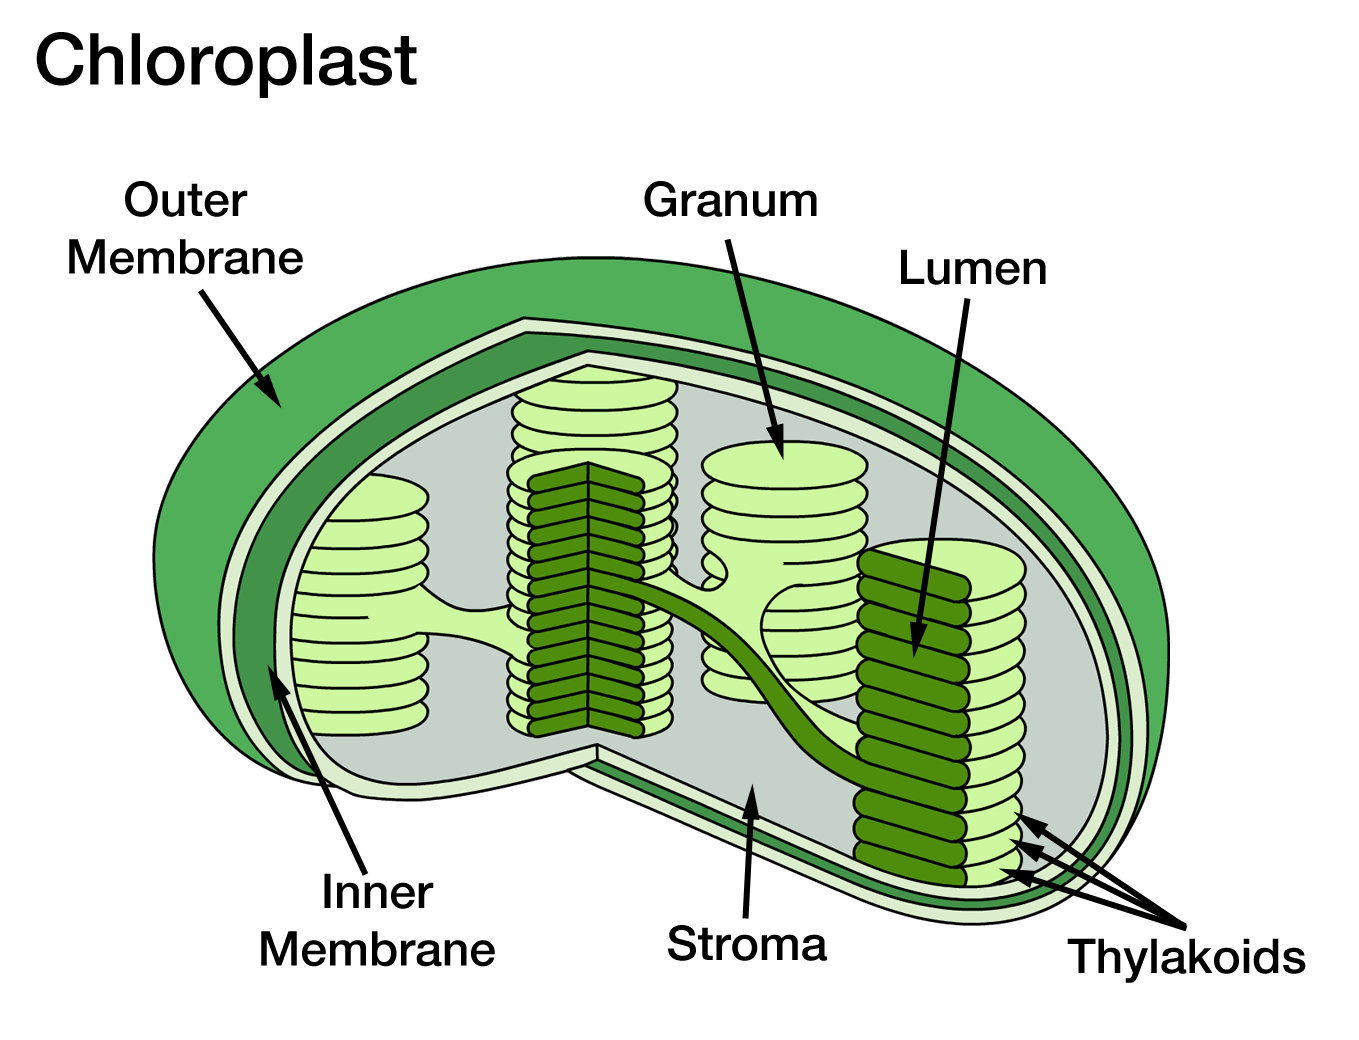
\includegraphics[scale = 0.25]{chloroplast.png}
        \label{Chloroplast}
    \end{figure}
    
    \begin{figure}[h!]
        \caption{Electron Transport between Photosystem II 
                 and the Cytochrome Complex. Plastoquinone (PQ) 
                 carries electrons from photosystem II along with 
                 protons from the stroma. The cytochrome complex 
                 oxidizes plastoquinone, releasing the protons in 
                 the thylakoid lumen that drive ATP synthesis}
        \centering
        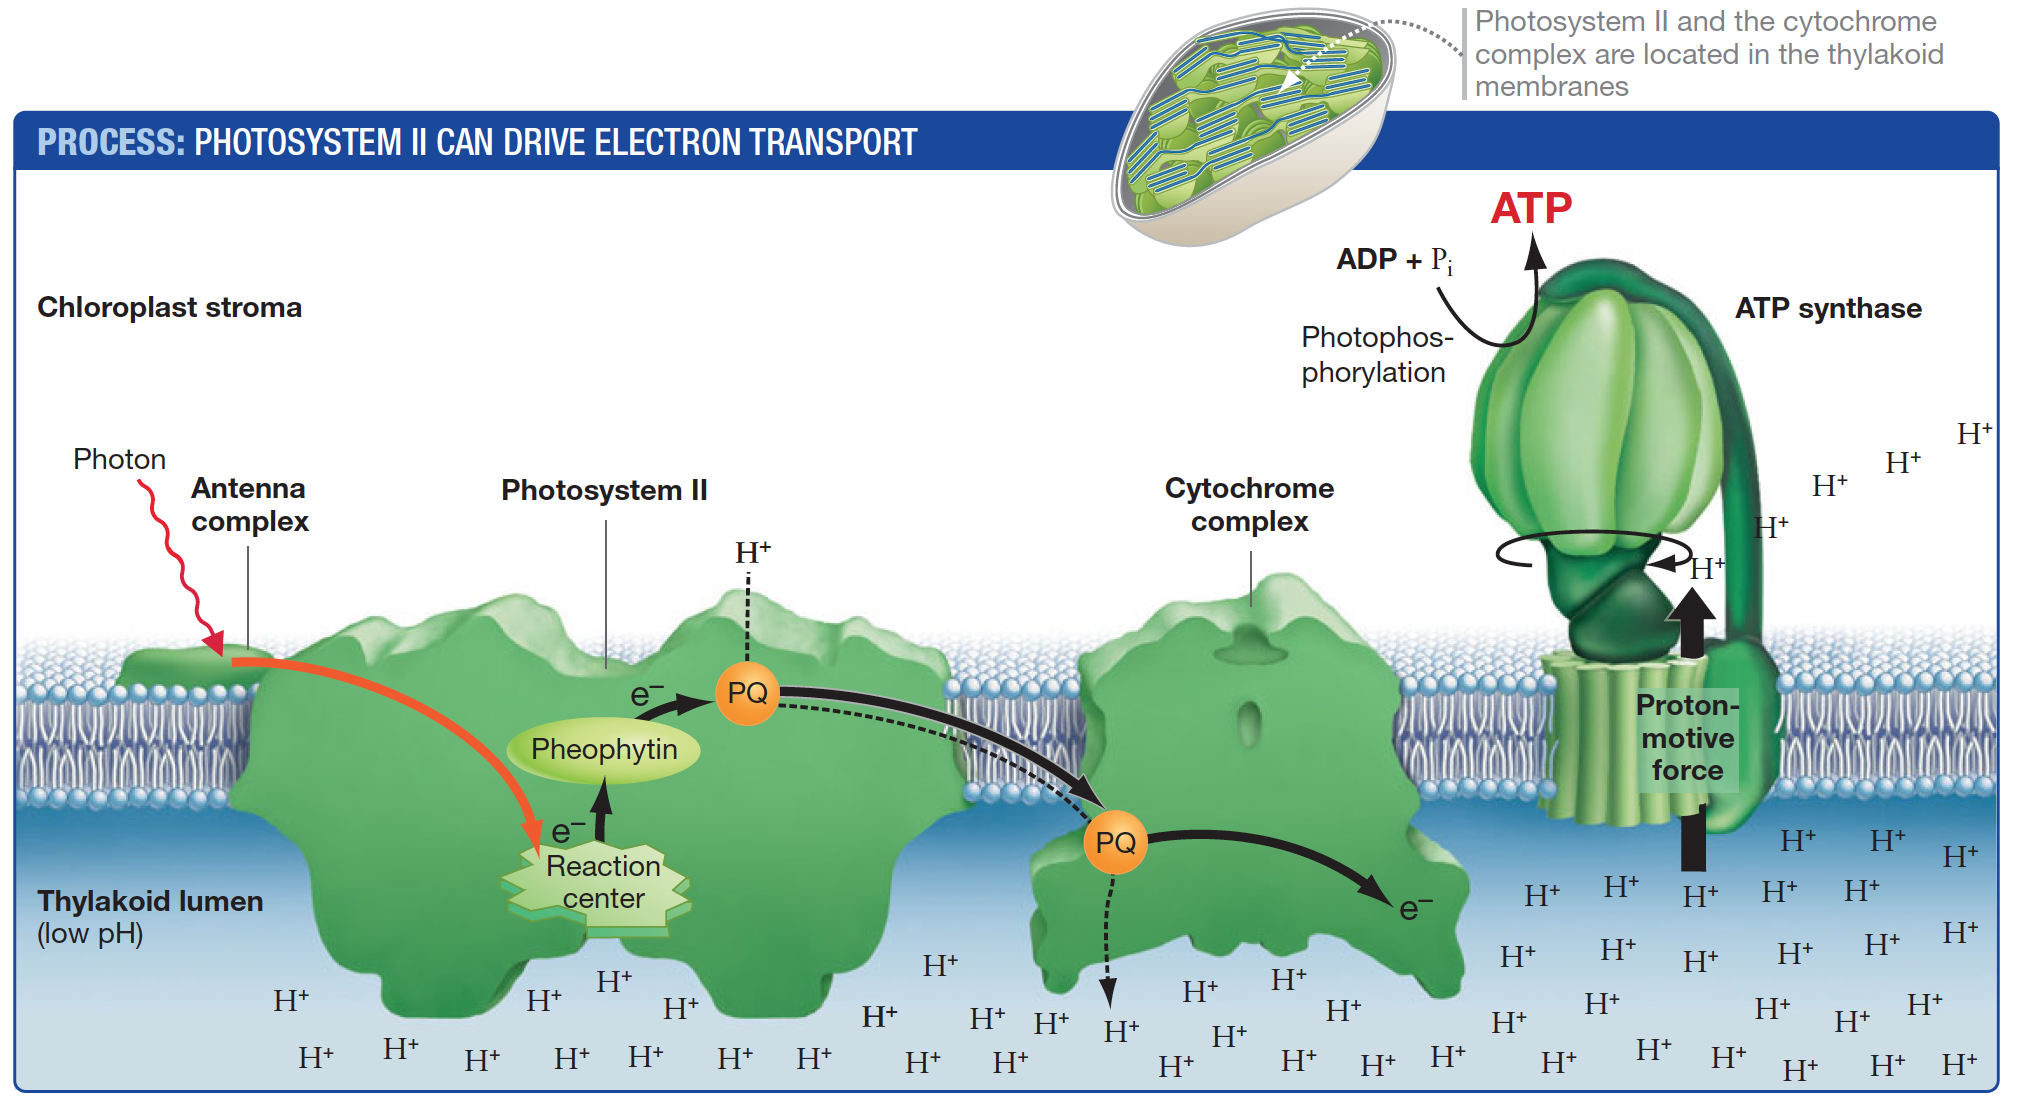
\includegraphics[width=\textwidth]{photosystem.png}
        \label{photosystem}
    \end{figure}
	
	In the light-dependent reactions, or "light reactions", ATP and NADPH 	
	are synthesized when photons activate the reaction regions
	on the thylakoid membranes in the chloroplasts. ATP and NADPH
	are the chemical energy used later in the light-independent or "dark"
	reactions to drive the production of sugars from $CO_2$ and water.
	As shown in Figure \ref{Chloroplast}, the lumen is the inside 
	of the thylakoid membrane, and the stroma is outside the thylakoid 
	membrane, where the light-independent reactions take place. The 
	thylakoid membrane contains some integral membrane protein complexes 
	that can catalyze the light reactions. There are four main protein 
	complexes in the thylakoid membrane: Photosystem I (PSI), 
	Photosystem II (PSII), Cytochrome b6f complex, and ATP synthase. 
	These four complexes interact with each other to eventually create 
	the products ATP and NADPH. The two photosystems absorb light energy 
	through chlorophylls pigments. The light reactions begin in PSII, 
	when the reaction center of PSII absorbs a photon, an electron in 
	this chlorophyll molecule obtains a higher energy level and is 
	transferred to another molecule creating a chain of reduction-oxidation 
	reactions, called an electron transport chain (ETC). The ETC goes from 
	PSII to cytochrome b6f to PSI, where the electron gets the 
	energy from another photon and is transferred to the final 
	electron acceptor, NADP. This drives oxygenic photosynthesis 
	where water is photolyzed and generates oxygen. ATP synthase then
	catalyzes Cytochrome b6f to create ATP in a process called 
	photophosphorylation.
	
	In summary, the composition of the light reactions 
	forms the chemical equation:	
	\begin{align}
	    2 H_2O + 2 NADP + 3 ADP + 3 P_i + light &\rightarrow
	    2 NADPH + 2 H^+ + 3 ATP + O_2
	\end{align}


    
     \begin{figure}[h!]
        \caption{Carbon Dioxide Is Reduced in the Calvin Cycle. 
                 The number of reactants and products resulting from 
                 three turns of the cycle are shown. Of the six G3Ps 
                 that are generated during the reduction phase, one is 
                 used in the synthesis of glucose or fructose and the 
                 other five are used to regenerate RuBP. The 3 RuBPs 
                 that are regenerated participate in fixation reactions 
                 for additional turns of the cycle}
        \centering
        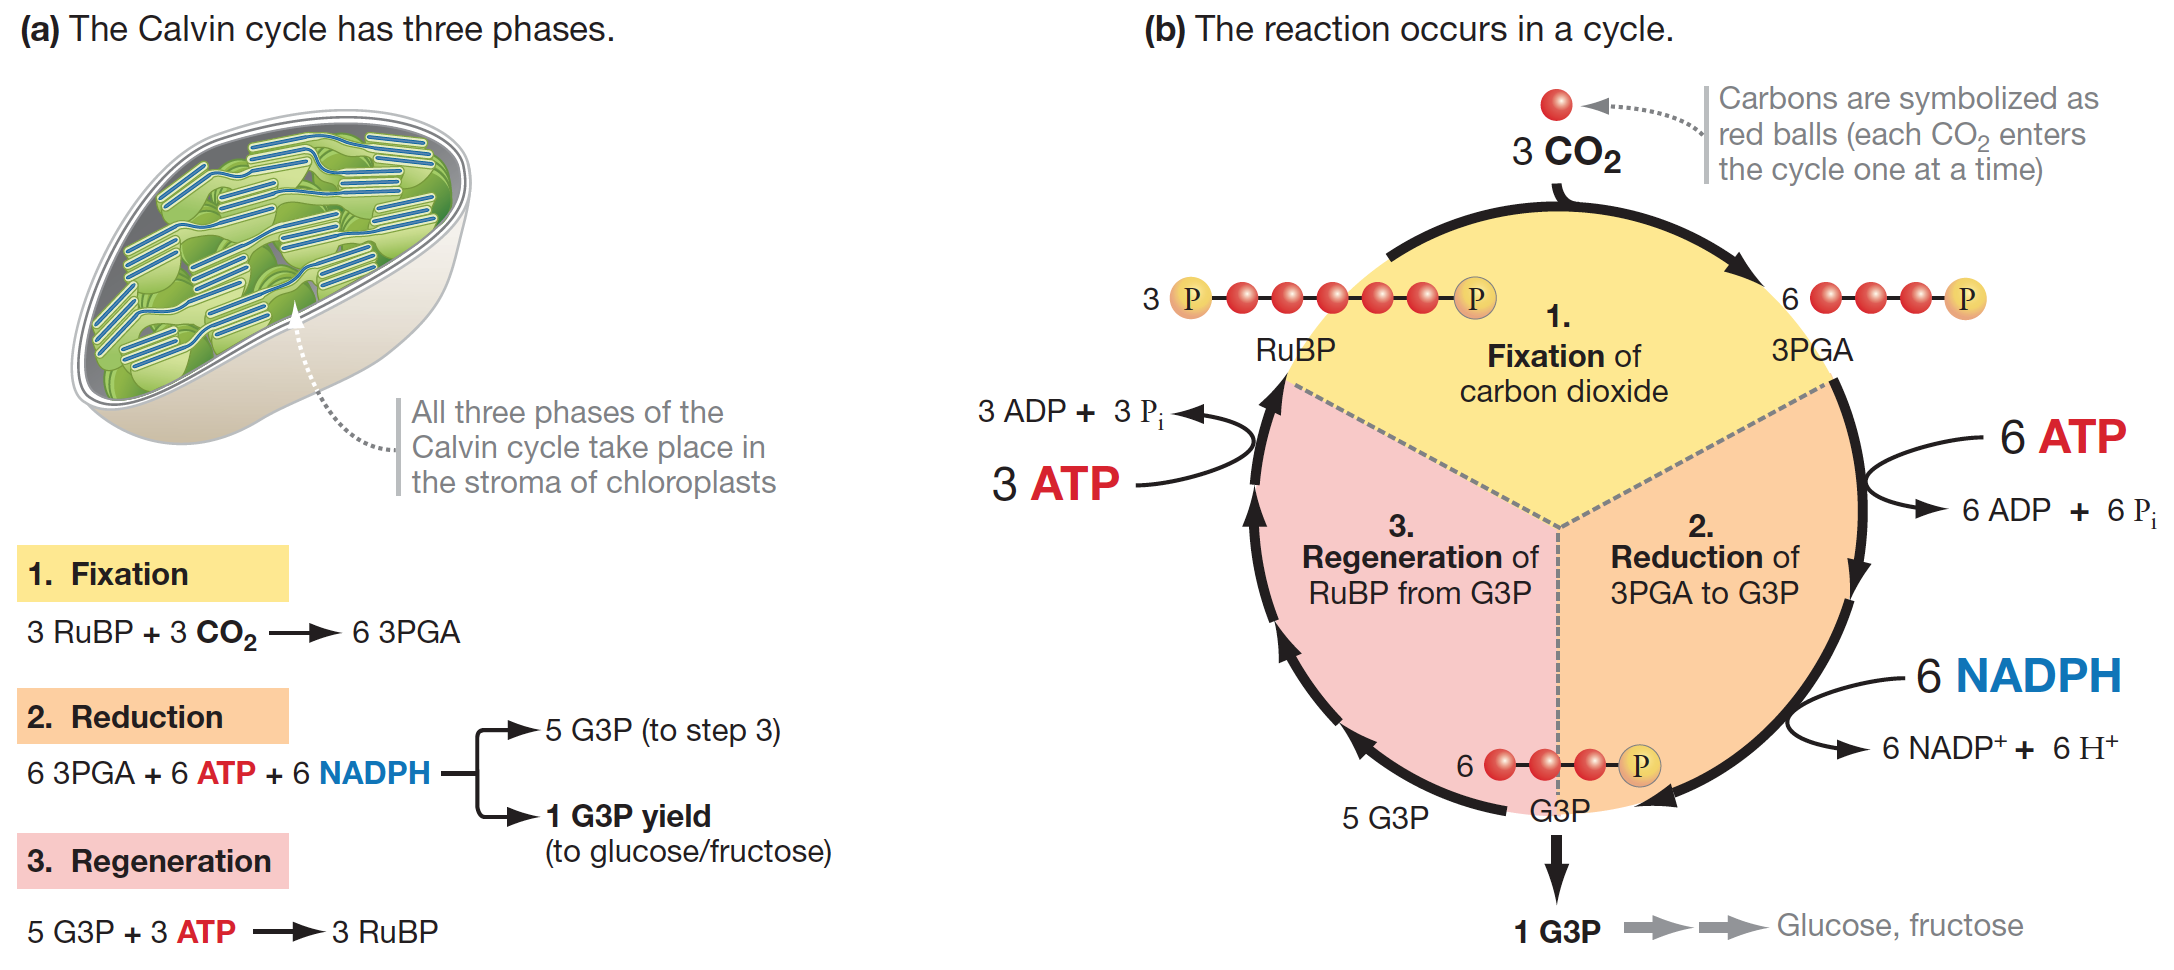
\includegraphics[width=\textwidth]{calvin.png}
        \label{CalvinCycle}
    \end{figure}
    
    In the dark reactions, carbon is removed from the $CO_2$ in the air
    and turned into glucose in a process called the Calvin cycle. 
    As shown in Figure \ref{CalvinCycle}, there are three phases in the Calvin 
    cycle: fixation, reduction, and regeneration. First, in the fixation 
    phase of the Calvin cycle, a $CO_2$ molecule is integrated into 1 
    of 2 three-carbon molecules (glyceraldehyde 3-phosphate or G3P), 
    where it uses up 2 ATPs and 2 NADPHs, both produced in the light 
    reactions. Next, the reduction phase, of the Calvin cycle is to 
    regenerate RuBP. Costing 3 ATPs, 5 G3Ps produce 3 RuBPs. Since 
    each CO2 molecule produces 2 G3Ps, 3 CO2 molecules produce 6 G3P 
    molecules, of which 5 are used to regenerate RuBP, leaving a net 
    gain of 1 G3P molecule per 3 CO2 molecules. Finally, in the 
    regeneration phase, of 6 G3Ps produced, 5 are used to make 3 RuBPs, 
    with only 1 G3P available for subsequent conversion to hexose. 
    This requires 9 ATPs molecules and 6 NADPHs per 3 CO2 
    molecules\cite{carbon_path}.
    
    This complex series of reactions can by summarized as     
    \begin{align}
        3 CO_2 + 9 ATP + 6 NADPH + 6 H^+ &\rightarrow 
        C_3H_6O_3-P_i + 9 ADP + 8 P_i + 6 NADP + 3 H_2O
    \end{align}


   
    
    \begin{figure}[h]
        \caption{ In the light-capturing 
                  reactions of photosynthesis, light energy is 
                  transformed to chemical energy in the form of 
                  ATP and NADPH. During the Calvin cycle, the ATP 
                  and NADPH produced in the light-capturing reactions 
                  are used to reduce carbon dioxide to carbohydrate. 
                  }
        \label{reactionsummary}
        \centering
        \begin{subfigure}[b]{0.35\textwidth}
            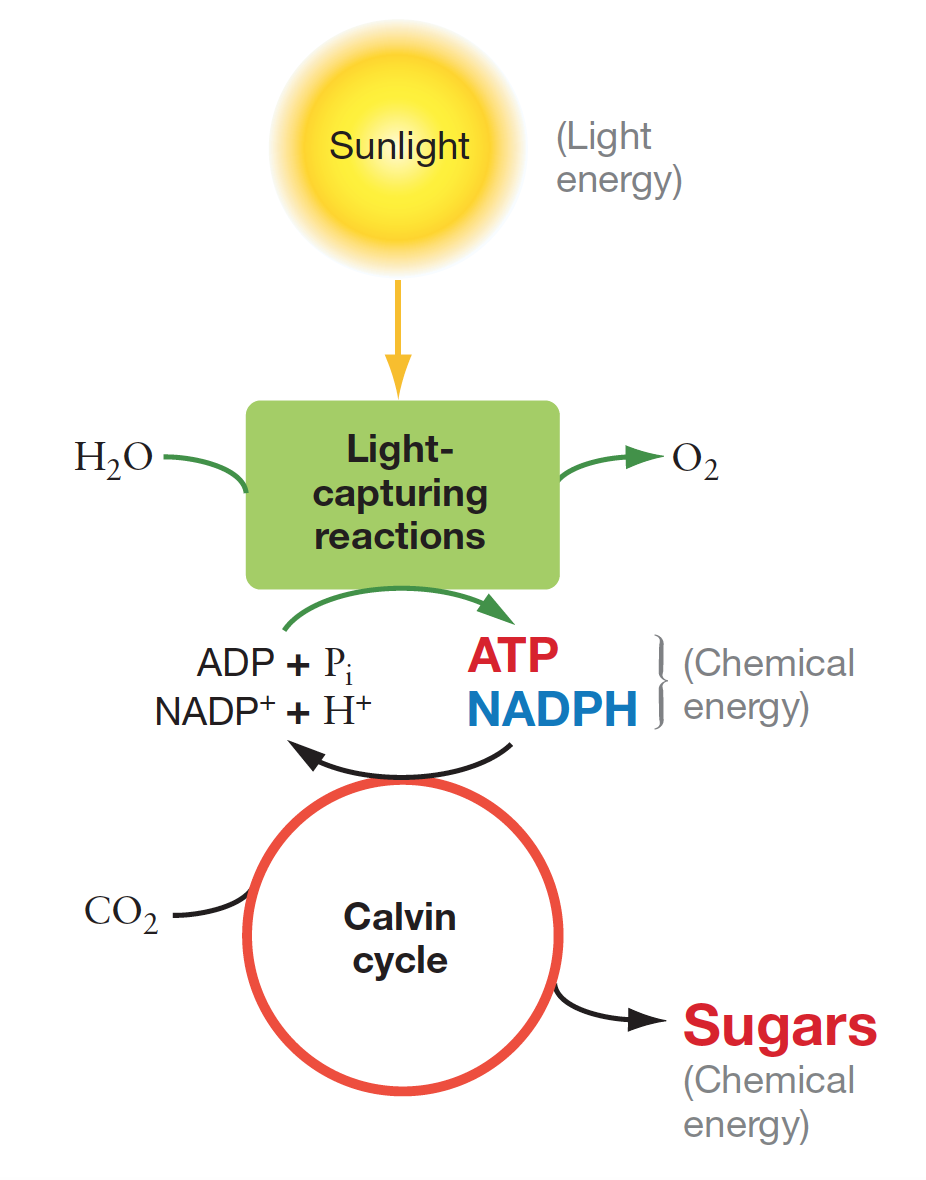
\includegraphics[width=\textwidth]{photosummary.png}    
            \caption{Photosynthesis has two linked components}
            \label{reactionsummary_a}
        \end{subfigure}
        \begin{subfigure}[b]{0.6\textwidth}
            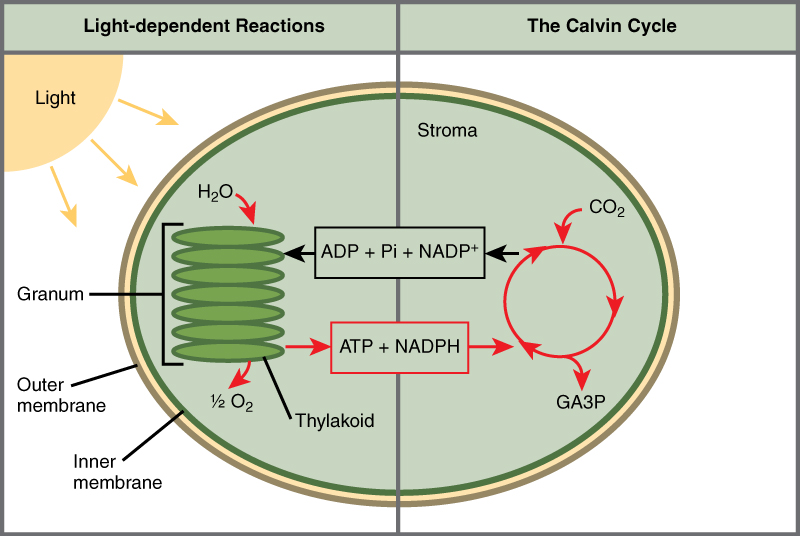
\includegraphics[width=\textwidth]{photocompartments.jpeg}
            \caption{Compartmentalization of photosynthesis}
            \label{reactionsummary_b}
        \end{subfigure}
    \end{figure}
    
    The combination of the light and dark reactions of 
    photosynthesis is shown in Figure \ref{reactionsummary}(a). 
    In the light-capturing reactions of photosynthesis, light energy 
    is transformed to chemical energy in the form of ATP and NADPH. 
    During the Calvin cycle, the ATP and NADPH produced in 
    the light reactions are used to reduce carbon dioxide 
    to simple sugars. Figure \ref{reactionsummary}(b)
    demonstrates the location each reaction takes place.

    In summary, the entire photosynthesis reaction can be written 
    in the simplified form:    
    \begin{align}
        6CO_2 + 6H_2O + light \rightarrow C_6H_{12}O_6 + 6O_2
    \end{align}


    
    
    \newpage
    
    \subsection*{Similar and Related Modelling}

    The method that our model implemented is called Gillespie Algorithm 
    initially discovered by Dan Gillespie in 1976\cite{gillespie}. 
    Since popularized in 1977, the method has been implemented by many 
    researchers in various fields across natural sciences such as 
    chemistry and biology\cite{gillespie_wiki}. One of the interesting 
    applications of Gillespie algorithm is exemplified in 
    An implementation of the Gillespie algorithm for RNA kinetics with 
    logarithmic time update by Eric C. Dykeman\cite{dykeman}. 
    In this paper, Dykeman built KFOLD method upon Gillespie algorithm to 
    select the samples of RNA molecules and predict folding kinetics. 
    By using the Gillespie algorithm, the KFOLD method is able to 
    compute a fixed number of changes at a low computational cost.
    
    Different from the above method which implements Gillespie
    algorithm to compute for chemical substances, there are also
    applications in many other fields. In Temporal Gillespie Algorithm:
    Fast Simulation of Contagion Processes on Time-Varying Networks by
    Vestergaard Christian and Genois Mathieu\cite{vestergaard}, 
    the Gillespie algorithm expands into the time-varying networks 
    and deals with the probability under a time frame. It’s very 
    exciting to see that there emerged new areas where the Gillespie 
    algorithm can be used.
    
    Another related model is presented by Daniel Hallen and Robert
    Runberg, a mathematical modelling of natural and artificial
    photosynthesis\cite{hallen}. In their setup, they used  ordinary 
    differential equations based on concentration of molecules 
    to construct the model of natural photosynthesis, which is in 
    contrast to our model since ours focuses on single molecules 
    instead of the concentration. And for artificial
    photosynthesis, they modelled the part of photosynthesis II that has
    been constructed today but added missing parts with non existing
    molecules since there is no complete system of artificial photosynthesis.
    However, our project is mainly based on natural photosynthesis,
    so the artificial part in their model is less appealing for us.
    In their natural photosynthesis model, they described the dynamics
    of the complexes in terms of the dynamic probabilities of possible 
    states of those complexes, which is an interesting part that differs
    from ours but also gets work.   

    
    
	\section*{\large \textbf{Model}}
	
	In order to simulate the complex dynamics of photosynthesis, we need
	to make many simplifying assumptions. While both the light and dark
	reactions are themselves a complex network of reactions catalyzed 
	by an even more complex network of interacting proteins and enzymes,
	many of the underlying reaction rate coefficients are poorly understood.
	Rather than introduce a host of reaction parameters into our model, we
	consider the simplified two equation system
	
	\begin{align}
	    2 NADP + 3 ADP &\xrightarrow{k_l} 2NADPH + 3 ATP + O_2 \\
	    6 CO_2 + 18 ATP + 12 NADPH + &\xrightarrow{k_d}
        Glucose + 18 ADP + 12 NADP 	    
	\end{align}
	
	These equations are slightly different than equations (1) and (2).
	In both equations, we've removed the hydrogen ion $H^+$, inorganic
	phosphate $P_i$, and water $H_2O$ terms. These chemical species are
	in overwhelming abundance in all regions of the chloroplast and
	therefore play no role in limiting the rates of these reactions.
	We've also removed the explicit dependence on light from the 
	reaction.  Instead, we can think of the rate coefficient $k_l$ as 
	a function of the light intensity. Setting $k_l = 0$ effectively 
	shuts off the light reaction allowing us to control the reaction
	rate quite efficiently.
	
	We've also doubled the number of reactants and products in our dark
	reaction equation, Eq.(5).  This allows us to ignore the complicated 
	branching of G3P that occurs in the transition between the reduction 
	and regeneration portions of the Calvin cycle and instead focus on 
	the eventual output, glucose.  
	
	The stochastic simulation of the Gillespie algorithm is especially 
	import for modelling biochemical reactions as the majority of biochemical 
	reactions occur at very specific locations, usually on the membrane of 
	some cell organelle.  Typical reaction modelling uses differential equations
	and continuous concentrations as the dynamic variables. The nonlinearity
	of the resulting equations coupled with the inhomogeneous distribution of 
	reaction sites contradicts the assumptions required for the continuous 
	technique to be accurate, especially in limiting cases\cite{gillespie}.
	
	Here instead we consider the actual number of molecules as our dynamic
	variables. To enforce some approximation of the locality requirement,
	we also use a compartment model for the chloroplast as seen in Figure 
	\ref{compartment}. In this model, we have subpopulations of the reactants
	in the different compartments and so we must also consider diffusion
	between the compartments. 
	
	This introduces the new model parameters $K_m$
	and $K_r$ which are the diffusion coefficients across the chloroplast 
	membrane (between inside and outside) between the interior and reaction
	regions, respectively.  Additionally we consider the $CO_2$ and $O_2$
	concentrations outside the chloroplast to be model parameters as they
	serve as a proxy for the makeup of the air the plant is growing in. 	
	
	\begin{figure}[h]
        \caption{Compartment Model of the Chloroplast}
        \centering
        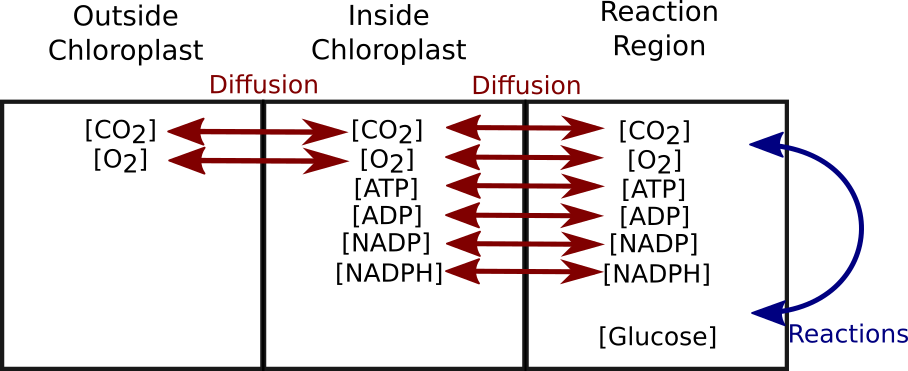
\includegraphics[width=\textwidth]{compartment.png}
    \label{compartment}
    \end{figure}
    
    To develop our model we start from the typical differential equation
    model with the interpretation of these equations as instantaneous 
    rate equations. By computing the individual reaction rates at each 
    time step of interest and by assuming reactions occur as a Poisson
    process, we can generate a joint probability distribution over
    time intervals and reactions. We then draw an update interval and a
    particular reaction from this distribution and use them to update
    the number of reactants in the system. This process is repeated
    until we're satisfied with the output results.
    
    Lets consider each piece of this process in turn.  First we look
    at the rate calculation step.  This comes from the normal differential
    equation reaction modelling. We denote the concentration of a reactant
    $X$ as $[X]$.  Then the reactions produce the following rate equations
    
    \begin{align*}
        \textrm{Let}&\\
        a_l =& k_l\cdot[NADP]\cdot[ADP] \\
        a_d =& k_d\cdot[CO_2]\cdot[ATP]\cdot[NADPH] \\
        \textrm{then}&\\
        \frac{d[NADP]}{dt}_r &= -2\cdot a_l + 12 \cdot a_d \\
        \frac{d[ADP]}{dt}_r &= -3\cdot a_l + 18 \cdot a_d \\
        \frac{d[CO_2]}{dt}_r &= - 6 \cdot a_d \\
        \frac{d[ATP]}{dt}_r &= 3\cdot a_l - 18 \cdot a_d \\
        \frac{d[NADPH]}{dt}_r &= 2\cdot a_l - 12 \cdot a_d \\
        \frac{d[O_2]}{dt}_r &=  a_l\\
        \frac{d[Glucose]}{dt}_r &= a_d 
    \end{align*}
	
	These reactions all occur in the reaction region of Figure\ref{compartment}.
	These differential equations then only represent a portion of the total
	change in concentration since diffusion is also changing the species count
	in a region. If we consider, say, $ATP$ and it's diffusion, we have an 
	additional rate equation
	
	\begin{align*}
	    \Delta [ATP] &= [ATP]_c - [ATP]_r\\
	    \frac{d[ATP]_r}{dt}_d &= K\cdot\sqrt{\frac{T}{m_{ATP}}}*\Delta [ATP].
	\end{align*}

    Here $\Delta [ATP]$ is a rough approximation of the concentration gradient
    between $[ATP]_r$, the ATP in the reaction region and $[ATP]_c$ the ATP in 
    the body of the chloroplast. $K$ is the overall diffusion coefficient which 
    represents factors like the medium viscosity, membrane thickness, 
    geometry of the boundary between regions, etc.  $T$ is the temperature of the
    cell and $m_{ATP}$ is the mass of the $ATP$ molecule.  The equation says
    diffusion increases with temperature since molecules move more quickly, 
    decreases with mass since heavy molecules move more slowly, and increases with
    the difference in concentration between any two regions.  This equation is 
    fairly correct for the diffusion in the chloroplast, though it's probably a
    poor approximation of the osmosis across the chloroplast membrane.
    
    We won't repeat the remaining concentration equations here except to say they are
    identical in structure.  We use two separate diffusion coefficients.  One for 
    diffusion across the chloroplast membrane and the other for diffusion insided
    the chloroplast.  
    
    We then set 
    
    \begin{align*}
        D_X = \frac{d[X]}{dt}_d
    \end{align*}
    
    as the instantaneous rate for the diffusion reaction for species $X$.  
    The collection of these for each species as well as the light reaction
    rate $a_l$ and the dark reaction rate $a_d$ are collectively our reaction 
    rates.  For each reaction type, the mean time til that reaction occurs again
    is the inverse of the reaction rate.  Since the rate at which anything
    will happen is simply the sum of all the reaction rates, which we'll denote
    by $\lambda$, we also can write the mean time until any reaction occurs as   
        
    \begin{align*}
        \tau_m = \frac{1}{\lambda}    
    \end{align*}
    
    Then, under the assumption of a Poisson process, it's fairly straightforward
    to pick the next most likely reaction and the amount of time until
    the reaction occurs. For the time, we have
    
    \begin{align*}
        \tau = \frac{1}{\lambda}\log(\frac{1}{U_1})
    \end{align*}
    
    for $U_1$ drawn uniformly from the unit interval.  Likewise, if we denote
    the individual reaction rates as $a_i$ we can select one based on the
    relative reaction rates by choosing a random variable
    
    \begin{align*}
        r = lambda*U_2
    \end{align*}
    
    which gives for $U_2$ drawn uniformly from the unit interval. This gives us
    a random variable in the range $(0, lambda)$  which we can use to select
    the next reaction $j$ by finding $j$ such that
    
    \begin{align*}
        \sum\limits_0^{j-1} \leq r \leq \sum\limits_0^j
    \end{align*}
    
    We then update the current time step, the number of reactants in all compartments,
    and go back to the beginning.
    
    The update steps are performed by keeping matrices to store the reactant/reaction
    combinations as well as the number of molecules used in each reaction.  Implementation
    details can be found in the appendix.
	
	\section*{\large \textbf{Results}}
	
	The first thing we sought to model was the normal operation of photosynthesis.
	We picked light and dark reaction rates to result in a steady state where none of
	the reactants hovered around zero.  We then produced a single day/night cycle
	to see how the system responded.
	
	\begin{figure}[h]
        \caption{Normal photosynthesis, with and without diffusion}
        \label{normal}
        \centering
        \begin{subfigure}[b]{0.45\textwidth}
            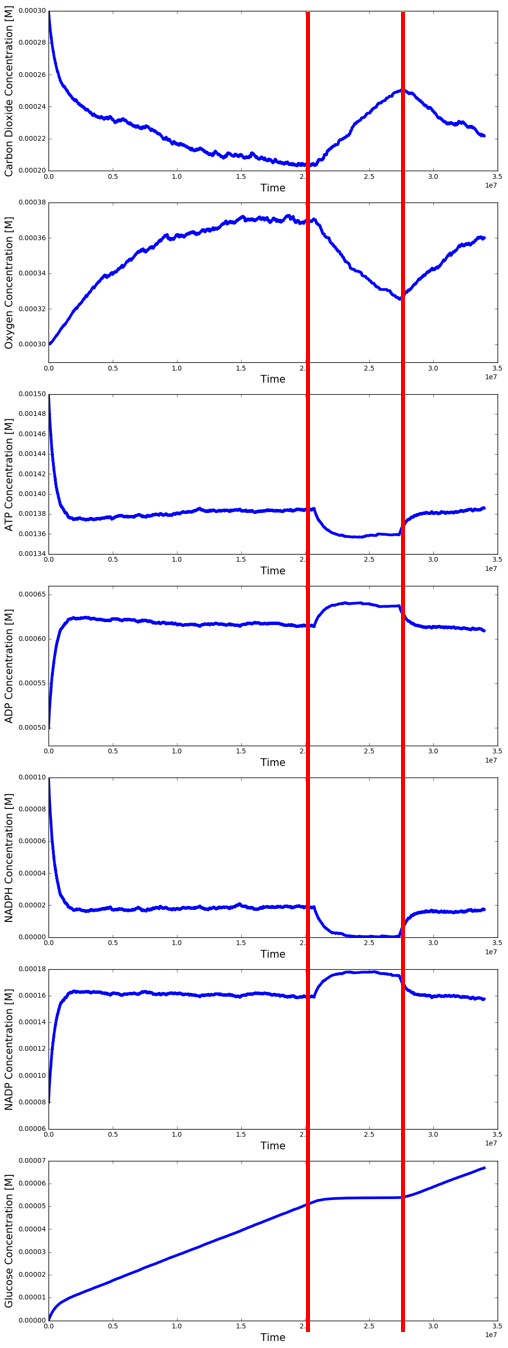
\includegraphics[width=\textwidth]{light_200_dark_500_on_off_on_labeled.png}    
            \caption{Limited diffusion}
            \label{normal_no_diff}
        \end{subfigure}
        \begin{subfigure}[b]{0.45\textwidth}
            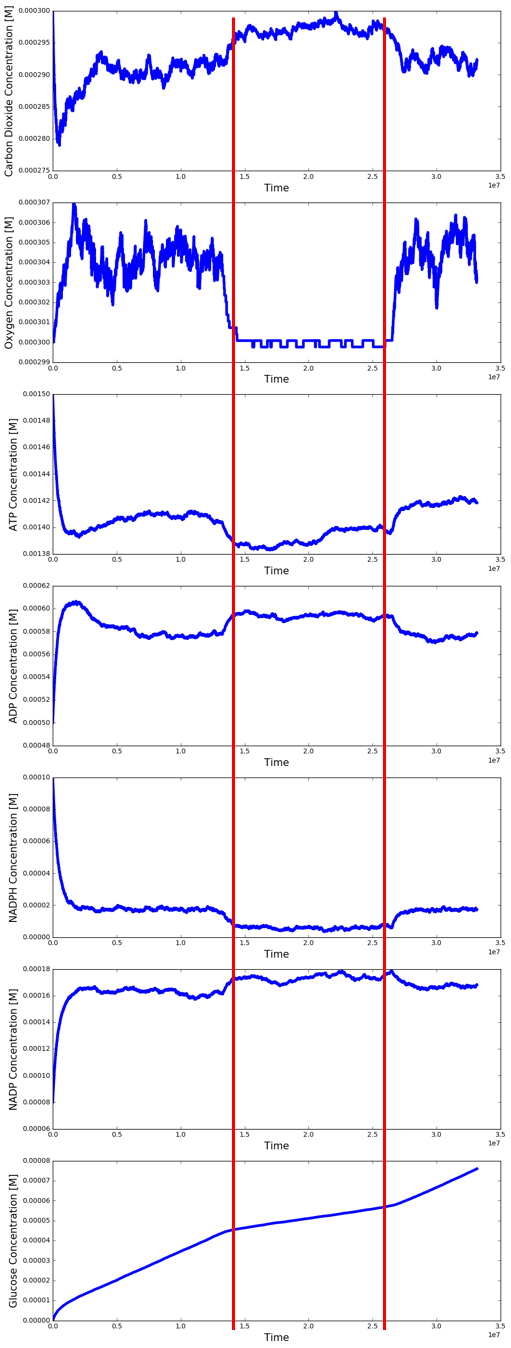
\includegraphics[width=\textwidth]{light_200_dark_500_on_off_on_with_diff_labeled.png}
            \caption{Abundant diffusion}
            \label{normal_diff}
        \end{subfigure}
    \end{figure}
    
    Figure \ref{normal} (a) shows the model with very limited diffusion across both the
    chloroplast membrane and between the reaction and non-reaction areas of the 
    chloroplast. This corresponds to the assumption that the diffusion rate
    of reactants is close to or smaller than the chemical reaction rates.
    This is not necessarily realistic, especially for the smaller molecules,
    but it produces easier to read graphs and gives us greater control over
    the state of the model.  In the figure, we see a pretty rapid shift from 
    the initial condition to a fairly stable steady state.  The $O_2$ and $CO_2$
    concentrations respond less strongly because even the relatively small
    diffusion constant affects them pretty strongly.  This steady state 
    is represented also by the linear slope in the glucose concentration
    indicating a consistent production rate.  At the first red line, the light
    reaction was turned off to simulate the onset of night time (here relatively short).  
    We can then see the rapid transition of all of the larger molecules to 
    a new steady state with diffusion-limited production of glucose.  Reintroducing
    the light source moves the system back into its previous steady state, as we
    would hope. This robustness to input  and ability
    to reproduce the same state in response to the same inputs despite the any previous
    state history is a key feature of photosynthesis in the short term.
    
    In figure \ref{normal}(b) we see a result that mirrors that in the first subfigure,
    but with some important differences.  Of particular not is much more rapid 
    transitions between steady states for all the molecules.  In the right ratio
    to the reaction rates, diffusion pushes the species concentrations in a semi-
    random way to their equilibrium position more rapidly.  We also see the impact
    of diffusion on the glucose production.  Even in the dark, glucose is still
    produced at a reasonable rate due to the reserves of chemical energy distributed
    throught the rest of the chloroplast.  
    
    These results, along with those presented in the following section, indicated 
    that our model is qualitatively correct.	
	
	
	\section*{\large \textbf{Adjustments and Extenstions}}
	
	Despite all the efforts we made to maximize the realistic accuracy 
	of the photosynthesis system, we have to admit there are considerable 
	amount of necessary assumptions we made to simplify our model. For 
	example, we made the assumption that the concentrations of the CO2 
	and H2O are maintained inside intracellular space, which can be subject 
	to realistic variations in different organisms and atmospheric pressures. 
	Additionally, the concentrations of each reactants are different in 
	stroma, intracellular space, and lumen space. However, we did
	accounts for the difference in concentrations of different process 
	by adjusting our model and including the compartimization, which 
	greatly resembles the real biological system. The introduction of 
	diffusion decreases the error of the concentrations we used in each 
	step of our simulations from the real concentrations in measurements.		
	
	
	\subsection*{Low Light Photosynthesis}
	Furthermore, we can extend the model and take into consideration the absence of light or the night environment. Before we change the light and dark rate, the reaction reaches its steady state with light rate = 200 and dark rate = 500. In this condition, based on the reaction all of the reactants are consumed up so no more glucose can be produced and therefore the reaction reaches the steady state. We then changed the set dark rate to 500 to mimic the night environment. As shown in the Fig.\ref{lowlight}, the concentration of glucose increases dramatically and goes beyond the previous steady state after the red line. This result proves our expectation that the dark reaction is initiated after we set dark rate to 500 and the glucose is being produced again because the products in the light reaction, namely the ADP, starts to react with NADP in the dark environment and produce glucose so that the concentration of glucose exceeds that of the previous steady state.
	
	\begin{figure}[h!]
        \caption{Low Light Photosynthesis and Transisition}
        \centering
        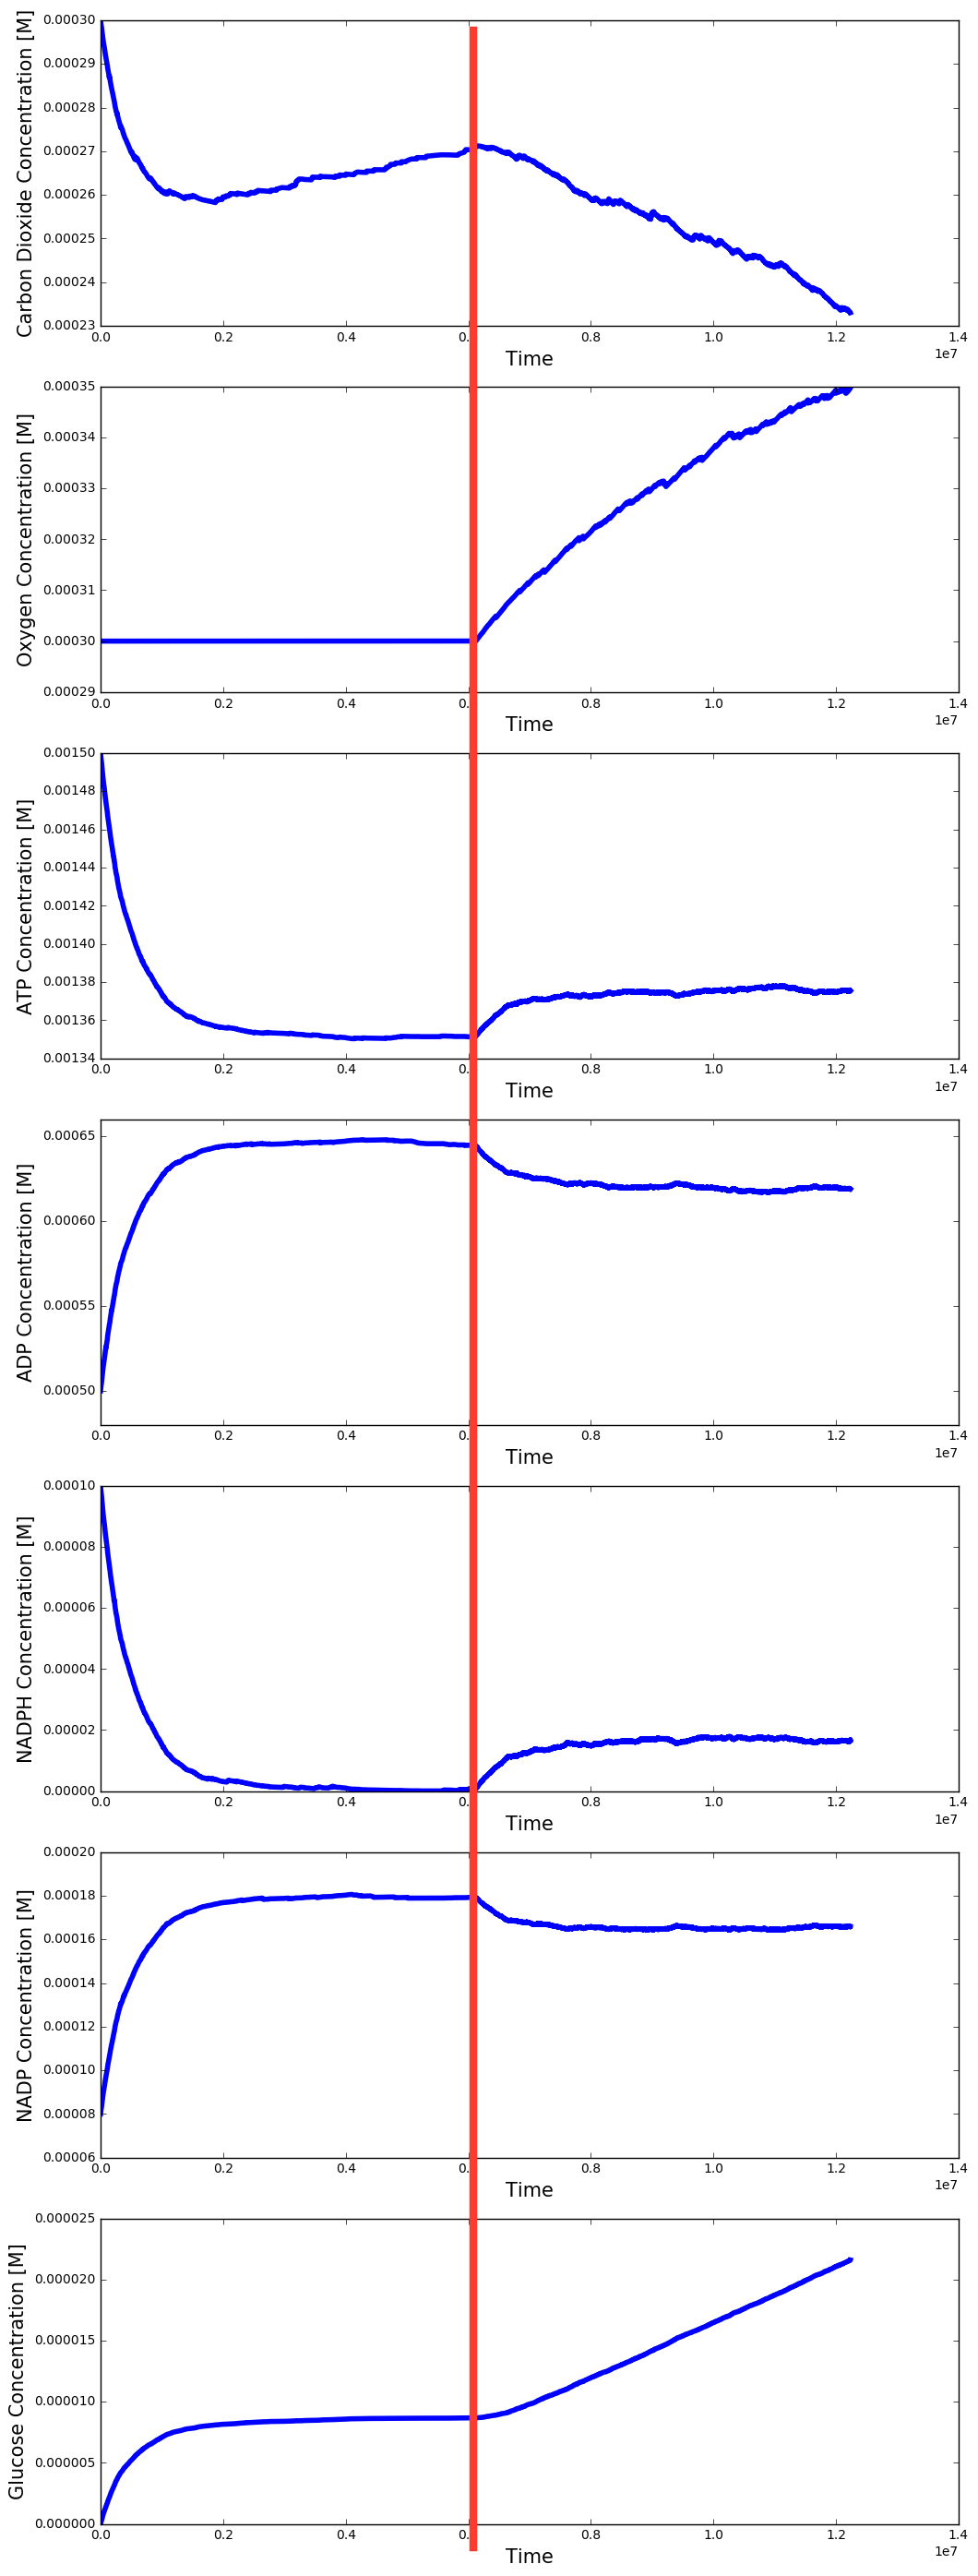
\includegraphics[height=\textheight]{final_pic.png}
        \label{lowlight}
    \end{figure}
	
	
	
	\subsection*{Calvin Cycle-limited Photosynthesis} For the condition that dark reaction is shifted off at the beginning, we firstly adjusted the light reaction rate = 500, then we shift the dark reaction on again with dark reaction rate = 500 as well. And we get the following graph. Before we shift dark reaction on, the simulation reached its steady state, which is the segment before the red line. In the steady state, the concentration of ADP and NADP almost hits zero level, and there is no glucose to be produced. After the dark reaction is shifted on, the concentration of ADP and NADP is precipitously increased and reaches to a new steady state in short time. While the concentration of NADPH and ATP just greatly decreases and also reaches to a new steady state in short time. Moreover, the concentration of glucose goes up as well as the concentration of oxygen does after the dark reaction is shifted on. These results make sense and reasonable since the glucose is rightly the production of dark reaction, so when dark reaction is present, glucose is present and accumulating as well. And for oxygen, since the simulation reached steady state before the dark reaction is shifted on, the system has consumed up ADP and NADP, then the concentration of oxygen is limited since oxygen is the production of ADP plus NADP. While the dark reaction is shifted on, the concentration of ADP and NADP increases, so does the concentration of oxygen behave since ADP and NADP are present again and oxygen is accumulating as production.  
	
	
	
	\begin{figure}[h!]
        \caption{Calvin Cycle-limited Photosynthesis and Transition}
        \centering
        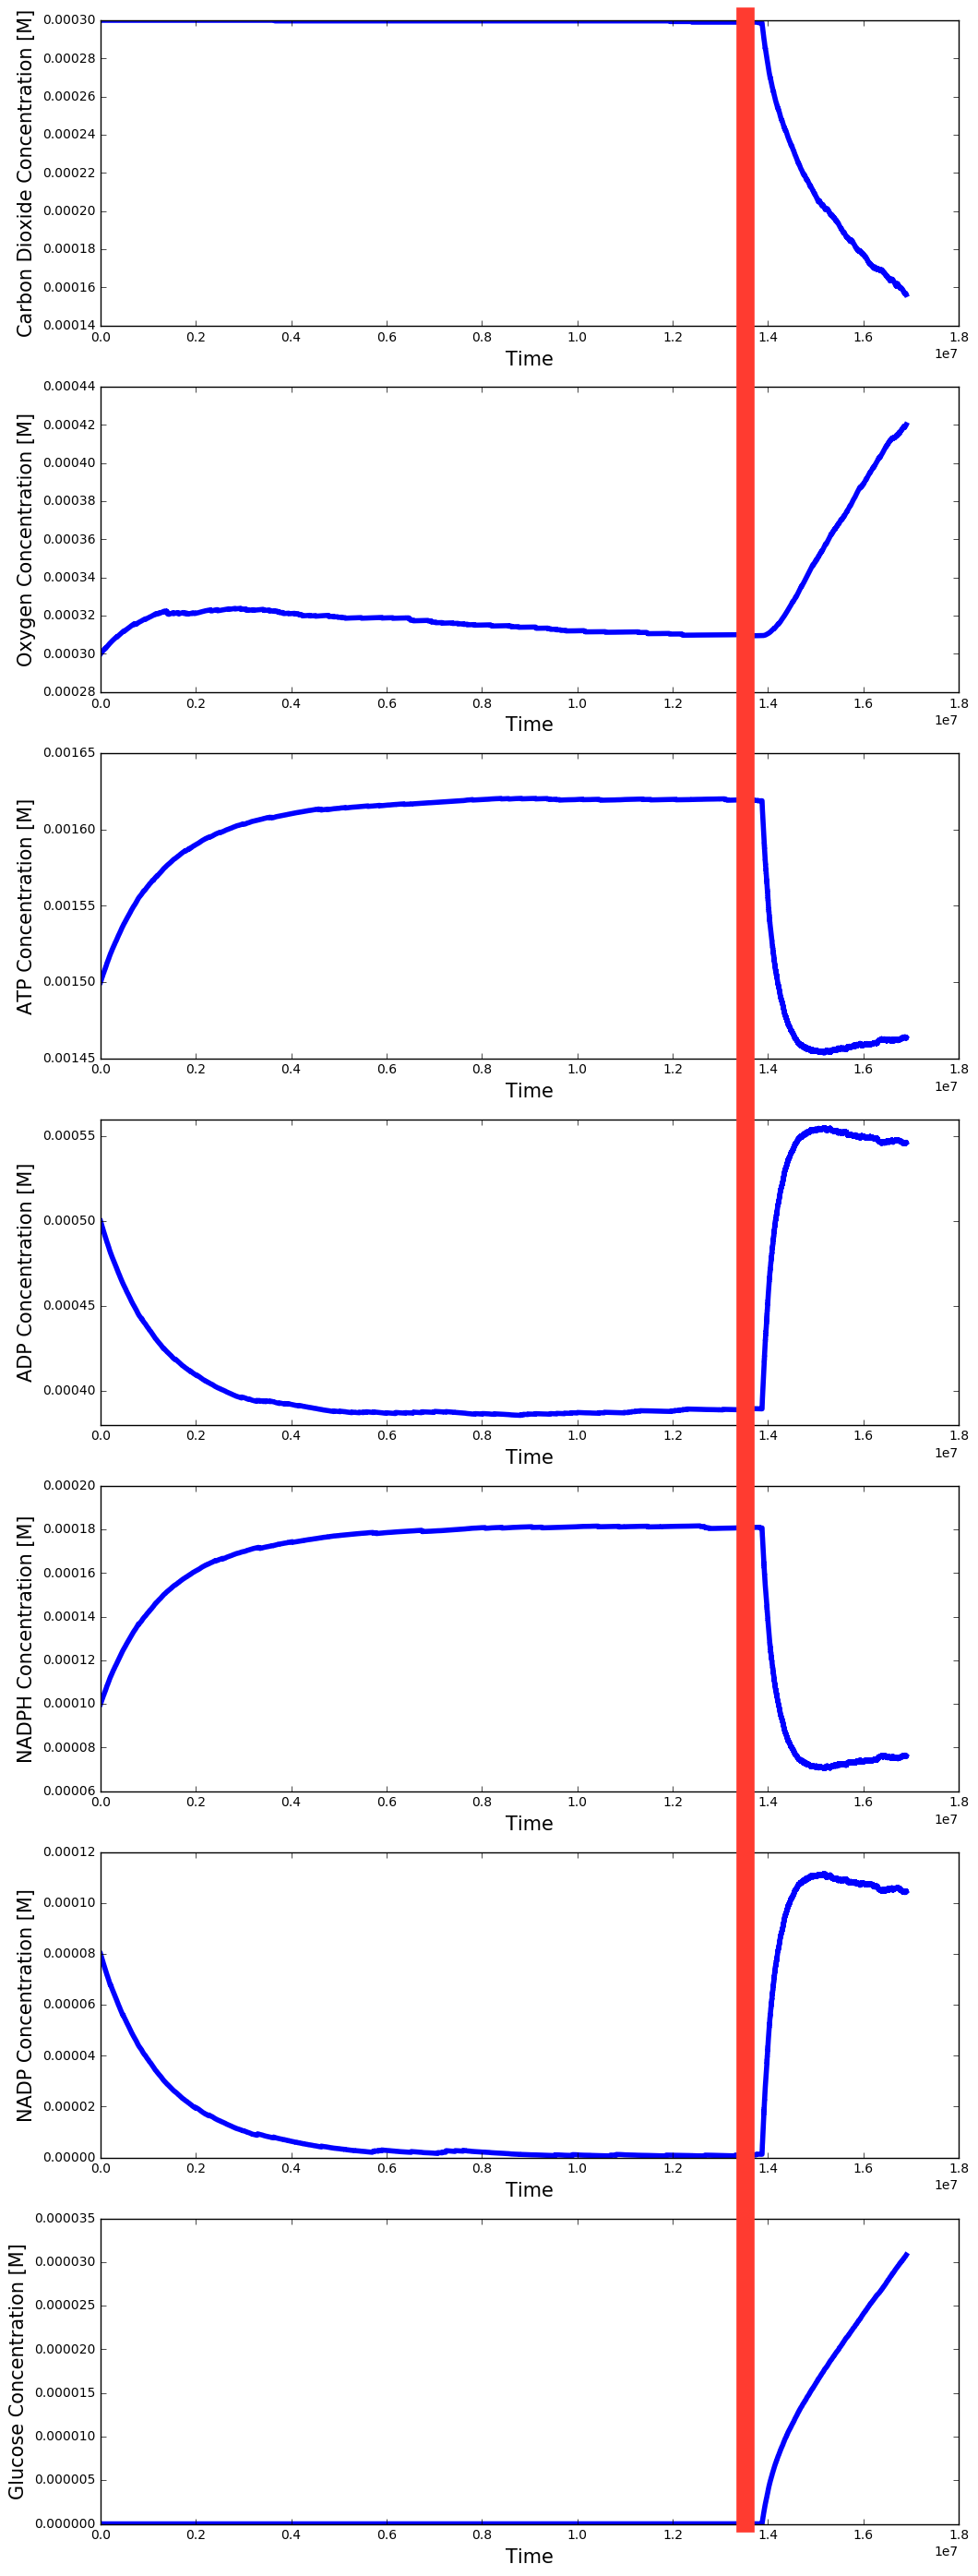
\includegraphics[height=\textheight]{light500(first)_dark500.png}
        \label{climit}
    \end{figure}
	

	\section*{\large \textbf{Conclusion}}
	
	From our exploration on modeling photosynthesis with Monte Carlos 
	simulation, we learned about the dynamics of the photosynthesis in 
	a mechanistic way. In our attempts, we learned to apply Gillespie’s 
	Monte Carlos simulation, while adjusting the reaction constants 
	calculation method in our discretion. More importantly, we managed 
	to update our model and add more realistic elements into our model 
	by many trials and errors based on the output we collected each time. 
	
	From our attempts, we successfully verified that our model can correctly simulate the photosynthesis and generate the values of all parameters needed to reach steady state in the normal condition. We also found that our model works well and can simulate the reactions of photosynthesis even in the extreme variations such as completely-dark and completely-bright variations.
	
	Considering the potential application of our model to agricultural 
	prediction and management, as well as the knowledge and skills we 
	learned, we think our efforts are very worthwhile and rewarding.
	\nocite{*}
	\printbibliography	
	
	\newpage
	
	
	
\end{document}